\documentclass[lettersize,journal]{IEEEtran}
\usepackage[utf8]{inputenc}
\usepackage{amsmath,amsfonts}
\usepackage{algorithmic}
\usepackage{algorithm}
\usepackage{array}
\usepackage[caption=false,font=normalsize,labelfont=sf,textfont=sf]{subfig}
\usepackage{textcomp}
\usepackage{stfloats}
\usepackage{url}
\usepackage{verbatim}
\usepackage{graphicx}
\usepackage{cite}
\usepackage{booktabs}
\usepackage[acronym]{glossaries}
\usepackage[unicode=true,pdfusetitle,
 bookmarks=true,bookmarksnumbered=false,bookmarksopen=false,
 breaklinks=false,pdfborder={0 0 0},pdfborderstyle={},backref=false,colorlinks=true]
 {hyperref}
\hypersetup{
 urlcolor=blue, linkcolor=black}
\hyphenation{op-tical net-works semi-conduc-tor IEEE-Xplore}

\global\long\def\BDsites{\textsf{BD\_sites}}

\title{Adaptative neigbouring methods applied to telephonic base stations}
\author{Paul MÉHAUD, Brendan SÉVELLEC}

\makeglossaries

\newacronym{arcep}{ARCEP}{French Regulatory Authority for Electronic Communications and Posts}
\newacronym{anfr}{ANFR}{French National Frequency Agency}

\begin{document}
\maketitle

\begin{abstract}
  The field of telecommunication represents a gigantic mine of information, the smartphone penetration rate being 69\%
  in 2023 in the world, and 97\% in France. Therefore, the collected datas represent a big opportunity for telecommunication
  companies to predict their customers behaviour for internal or marketing purposes. Thus, it is primordial for these companies
  to be able to determinate if a user is moving. For that, it is necessary to understand the neighbouring relationships between the 
  telephonic base stations. This article aims at comparing different method, ellaborated in order to adaptively detect these
  relationship between telephonic base stations given their geographical positions.
\end{abstract}

\section{Introduction}
    \IEEEPARstart{T}{his} article is the continuation of the work done by Delphine Paquiry in this paper \cite{art_del_paq}.
    It aims at discovering the neighbouring relationships between base stations from their geographical positions, using a 
    measure of the density of base station.

    For that, it is necessary to describe and analyse the databases that have been used during the research, then to present 
    the different appoaches that always consist of these steps : establish a first neighbouring graph, compute the base station 
    densities and filter this graph with different criteria using this information. The final step is to present the results
    of the different approches and conclude.
\section{Related works}

\section{Databases}
    Several databases have been used in order to test the different aspects of the methods. However, one of
    them is directly necessary to the method itself.

    \subsection{Main database}

    This database \cite{main_database} contains all the information needed to the application of the method. It is from
    \acrfull{arcep}, which is a french national organisation that

    The fields that are being used here are the following :

    \begin{table}[!b]
        \centering
        \caption{Description of the dataset}
        \label{data_columns}
        \begin{tabular}{ll}
            \toprule
            \textbf{Column} & \textbf{Description} \\
            \cmidrule(lr){1-2}
            \textsl{BS\_anfr\_id} & \acrshort{anfr} base station ID \\ 
            \textsl{x, y, latitude, longitude} & Base station coordinates \\ 
            \textsl{nom\_reg, nom\_dep, nom\_com} & Additional location information \\  
            \textsl{site\_2g, 3g, 4g, 5g} & Technology used by the base station \\ 
            \bottomrule
        \end{tabular}
    \end{table}

\section{Finding potential neighbours}
\noindent When we are looking for neighbours, we need, at first, a list of potential neighbours for each base stations.
Here are the different methods we can use to solve this problem:

\subsection{Delaunay triangulation}
\noindent The Delaunay triangulation is named after Boris DELAUNAY for his work on it from 1934 [citer l'article].

The principle of this method is quite simple. Let $P$ be a set of points in the plane and $D(P)$ the triangulation we are looking for.
A triangle $t_i$ is in $D(P)$ if its circumcircle does not contain any point inside (it can contain points on the border).

However, a Delaunay triangulation is not unique.

You can find an illustration of this method in figure \ref{del_tri}.
\begin{figure}[!t]
    \centering
    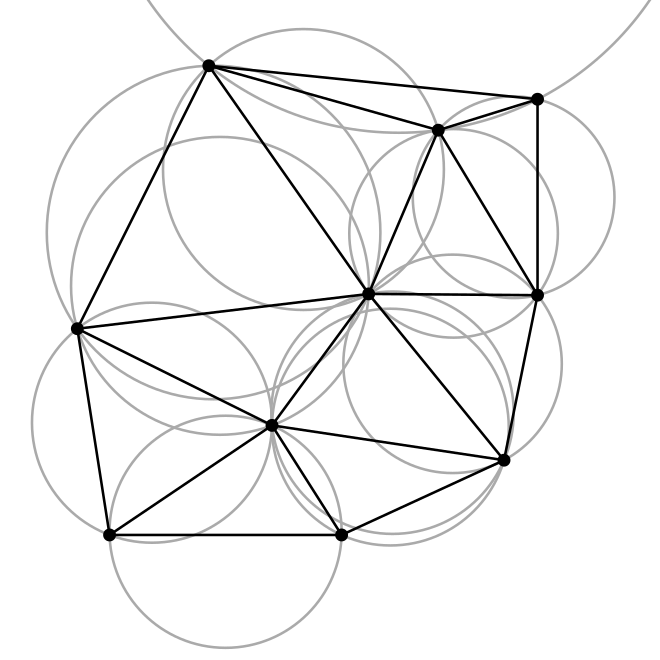
\includegraphics[width=2.5in]{images/illus_graphs/Delaunay_circumcircles_vectorial.svg.png}
    \caption{Example of a Delaunay triangulation}
    \label{del_tri}
\end{figure}

\subsection{Gabriel graph}
\noindent The Gabriel graph is a subgraph of a Delaunay triangulation. Thus, if the Delaunay triangulation is given, it can be found in a linear time. 

Gabriel graphs are named after K. Ruben Gabriel, who introduced them in a paper with Robert R. Sokal in 1969[citer].

The principle is really close to the one presented before. Let $G$

\subsection{$k$-NN graph}

\section{Results}

\section{Conclusion}

[Ouverture : prendre en compte les zazimuths]

\printglossary[type=\acronymtype]

\bibliographystyle{alpha}
\bibliography{./biblio.bib}

\end{document}


